\documentclass{article}
\usepackage[pagebackref]{hyperref}
\usepackage[dvipsnames,pdftex,fixpdftex]{xcolor}
\usepackage{tikz}
%\usetikzlibrary{decorations.pathmorphing}
\usepackage[hmargin=1cm,vmargin=1cm]{geometry}

\usetikzlibrary{arrows}
\usepackage{verbatim}

\begin{document}


% \tikzstyle{int}=[draw, fill=blue!20, minimum size=2em]
%\tikzstyle{init} = [pin edge={to-,thin,black}]

\begin{figure}
\centering
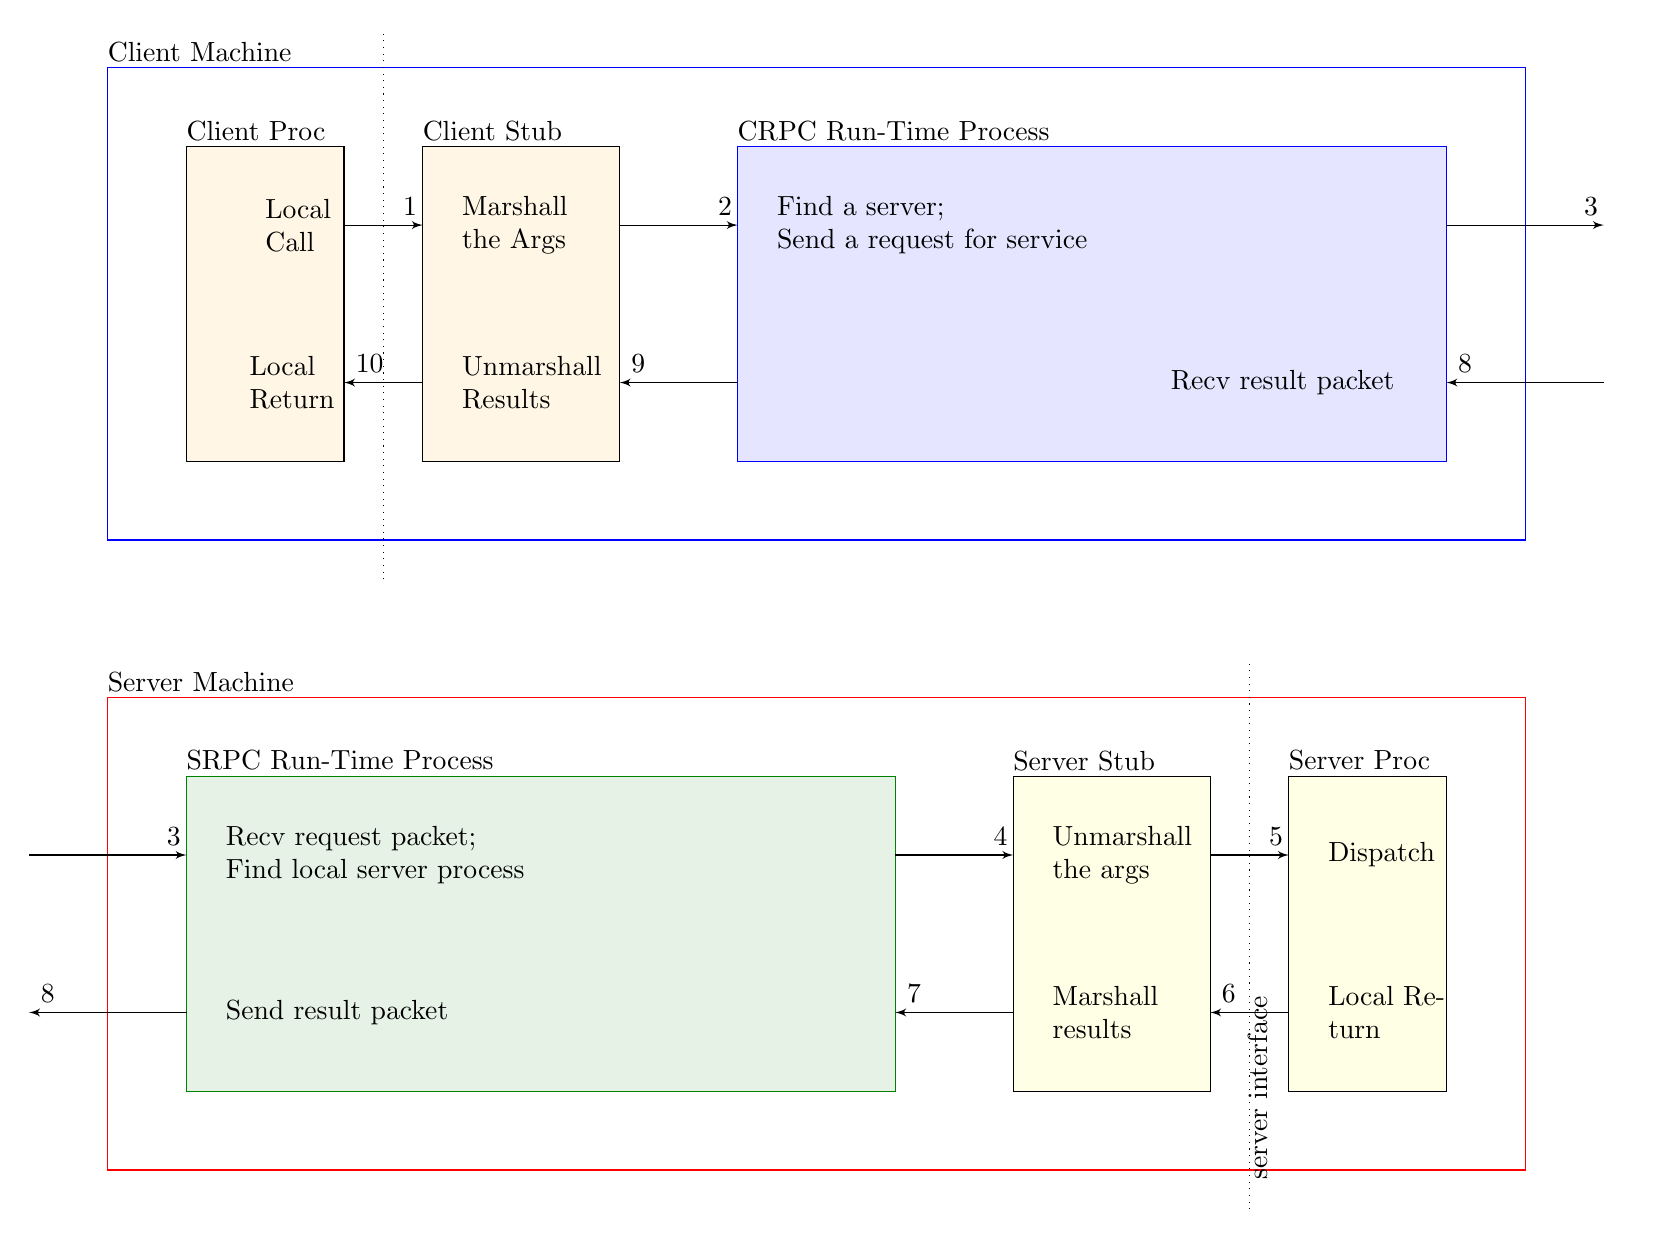
\begin{tikzpicture}[node distance=2.5cm,auto,>=latex']

% {Client Machine};
\begin{scope}
\draw [draw=blue] (0,0) rectangle ++(18,6);
\filldraw [fill=Orange!10] (1,1) rectangle ++(2,4);
\filldraw [fill=Orange!10] (4,1) rectangle ++(2.5,4);
\filldraw [draw=Blue,fill=Blue!10] (8,1) rectangle ++(9,4);

\node[text width=3cm] at (1.5,6.2) {Client Machine};
\node[text width=2cm] at (2,5.2) {Client Proc};
\node[text width=2cm] at (5,5.2) {Client Stub};
\node[text width=5cm] at (10.5,5.2) {CRPC Run-Time Process};


\node[text width=2cm] at (3,4) {Local\\Call};
\node[text width=2cm] at (2.8,2) {Local\\Return};
\node[text width=2cm] at (5.5,4) {Marshall\\the Args};
\node[text width=2cm] at (5.5,2) {Unmarshall\\Results};
\node[text width=5cm] at (11,4) {Find a server;\\Send a request for service};
\node[text width=4cm] at (15.5,2) {Recv result packet};

\draw [->](3,4) -- (4,4) node[text width=5mm, above] {1};
\draw [->](6.5,4) -- (8,4) node[text width=5mm, above] {2};
\draw [->](17,4) -- (19,4) node[text width=5mm, above] {3};
\draw [->](19,2) -- (17,2) node[text width=-3mm, above] {8};
\draw [->](8,2) -- (6.5,2) node[text width=-3mm, above] {9};
\draw [->](4,2) -- (3,2) node[text width=-3mm, above] {10};
\draw [dotted] (3.5,-0.5) -- (3.5,6.5);
\end{scope}

% {Server Machine};
\begin{scope}[yshift=-8cm]
\draw [draw=red] (0,0) rectangle ++(18,6);
\filldraw [draw=Green,fill=Green!10] (1,1) rectangle ++(9,4);
\filldraw [fill=Yellow!10] (11.5,1) rectangle ++(2.5,4);
\filldraw [fill=Yellow!10] (15,1) rectangle ++(2,4);

\node[text width=3cm] at (1.5,6.2) {Server Machine};
\node[text width=2cm] at (16,5.2) {Server Proc};
\node[text width=2cm] at (12.5,5.2) {Server Stub};
\node[text width=5cm] at (3.5,5.2) {SRPC Run-Time Process};


\node[text width=2cm] at (16.5,4) {Dispatch};
\node[text width=2cm] at (16.5,2) {Local Return};
\node[text width=2cm] at (13,4) {Unmarshall\\the args};
\node[text width=2cm] at (13,2) {Marshall\\results};
\node[text width=5cm] at (4,4) {Recv request packet;\\Find local server process};
\node[text width=5cm] at (4,2) {Send result packet};

\draw [->](10,4) -- (11.5,4) node[text width=5mm, above] {4};
\draw [->](14,4) -- (15,4) node[text width=5mm, above] {5};
\draw [->](-1,4) -- (1,4) node[text width=5mm, above] {3};
\draw [->](1,2) -- (-1,2) node[text width=-3mm, above] {8};
\draw [->](11.5,2) -- (10,2) node[text width=-3mm, above] {7};
\draw [->](15,2) -- (14,2) node[text width=-3mm, above] {6};

\draw [dotted] (14.5,-0.5) -- (14.5,6.5)
 node[text width=3cm, rotate=90,pos=0.5,yshift=-1mm] {server interface};
\end{scope}


\end{tikzpicture}
\caption{RPC architecture}
\end{figure}

% (Drawn with LateX/TiKZ \url{http://www.texample.net/tikz/examples/})
\end{document}

